\chapter{Approximation}
{\parindent0pt
\underline{Purpose}: Approximate a general function by a class of simpler functions

There are two motivations for this:
\begin{enumerate}
    \item Decompose a complicated function into its constituent simpler functions, in order to manipulate the function more easily (e.g. differentiation, integration, storage, etc.)
    \item Recover a function from partial or noisy information (for example, we may have stored some values of the function in a table, or we may be observing or sensing the function at discrete times
\end{enumerate}

\underline{Applications}:
\begin{itemize}
    \item Signal compression and reconstruction (Fourier techniques)
    \item Data fitting (best line, best quadratic, ...)
    \item CAD representations of shapes
\end{itemize}
\emph{Note: Approximation goes beyond interpolation}

\section{Uniform approximation by polynomials}
Let us start by looking at polynomials again. This time, rather than interpolate at given fixed points, we will seek the best uniform approximation. \\

Given a function $f:[a, b] \rightarrow \mathbb{R}$ and a polynomial $p$, we measure the error between $f$ and $p$ in terms of an $L_\infty$ norm, that is,
\begin{equation*}
    ||f - p||_\infty = \max_{a \leq x \leq b}{|f(x) - p(x)|}
\end{equation*}

A good uniform approximation is one for which this error is small. Recall from Weierstrass' Theorem that (for continuous f), we can make this error arbitrarily small by choosing a polynomial $p$ of high-enough degree. \\

Let's restrict the degree of the polynomial \\

\underline{Def:} Let \underline{$\Pi_n$} consist of all polynomials of degree at most $n$ \\

\underline{Def:} The \underline{uniform distance} of $f$ from $\Pi_n$ is the smallest error achievable using polynomials in $\Pi_n$.
\begin{equation*}
    d (f, \Pi_n) = \min_{p \in \Pi_n}{||f - p||_\infty}
\end{equation*}

The goal in best uniform approximation is to find a polynomial $p$ that actually achieves this minimum possible error. \\

The following theorem helps us: \\

\fbox{\parbox{\textwidth}{%
\underline{Theorem}: A function $f$ which is continuous on $[a, b]$ from $\Pi_n$ \\

The polynomial $p \in \Pi_n$ is the best uniform approximation to $f$ on $[a,b]$
\begin{align*}{\text{if and only if}}\end{align*}

There are $n + 2$ points $a \leq x_0 \leq ... \leq x_{n+1} \leq b$ such that \\

\begin{equation*}
    (-1)^2 [f(x_i) - p(x_i)] = \epsilon || f - p ||_\infty ~~~ i = 0, ..., n+1
\end{equation*}
where $\epsilon = signum[f(x_0) - p(x_0)]$\\

(Here $x_0 = a$ and $x_{n+1} = b$ in case $f^{(n+1)}(x)$ does not change sign on $[a,b]$)}%
}\\

In other words, with alternating sign at $n+2$ points, the difference between $f$ and $p$ is precisely equal to the $L_\infty$ distance between $f$ and $p$. \\

The idea is the apply this theorem by constructing a polynomial $p$ that satisfies the alternating-error-condition. By the theorem, that polynomial is the best uniform approximation. \\

\underline{Ex.} Consider $f(x) = e^{x}~\text{on}~[-1, 1]$ \\

Let us construct the best uniform approximation to $e^x$ by a straight line over the interval $[-1, 1]$. \\

With $n=1$, the alternating-error-condition of the previous theorem tells us that qualitatively the best uniform approximation will look something like this.

\begin{figure}[H]
    \centering
    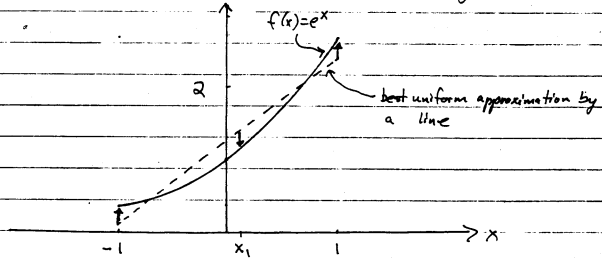
\includegraphics[width=0.9\textwidth]{figures/approximation_1}
    % \caption{Caption}
    \label{fig:approximation-1}
\end{figure}

The point is that there are three points $x_0 = -1$, $x_1 = ?$, $x_2 = 1$ at which the error $f(x) - p(x)$ is greatest, with equal magnitude and alternating sign. \\

The trick is to figure out what the point $x_1$ is. To do this, let's try to figure out what the theorem tells is in detail. \\

Let's write the polynomial as $p(x) = a + bx$ \\

(since $f''(x)$ does not change sign on $[-1, 1]$, we know that $x_0 = -1$ and $x_2 = 1$) \\

Computing errors we find that:
\begin{align*}
    e(x_0) &= f(x_0) - p(x_0) = f(-1) - p(-1) = \frac{1}{e} - a + b\\
    e(x_1) &= f(x_1) - p(x_1) = f(x_1) - p(x_1) = e^{x_1} - a - bx_1\\
    e(x_2) &= f(x_2) - p(x_2) = f(1) - p(1) = e - a - b
\end{align*}

The theorem says $e(x_0) = - e(x_1) = e(x_2) = ||f - p||_\infty$
\begin{align*}
    e(x_0) &= e(x_2) \\
    \frac{1}{e} - a + b &= e - a - b \\
    2b &= e - \frac{1}{e} \\
    b &= \frac{e - \frac{1}{e}}{2} \approx 1.1752
\end{align*}

This says that the slope of our best line must be the same as the average change of $f(x)$ over $[-1,1]$. \\

\underline{How do we choose a?}

Well, by definition $||f - p||_\infty$ is the maximum error between $f$ and $p$ over $[-1,1]$. It is equal to $-e(x_1)$. So the error function $e(x)$ must achieve a local extremum at $x = x_1$ \\

In other words, $e'(x_1) = 0$. We can use this fact to determine $x_1$.
\begin{align*}
    e(x) &= f(x) - p(x) = e^x - a - bx \\
    e'(x) &= e^x - b \\
    0 &= e^{x_1} - b \\
    x_1 &= \ln{b} \approx 0.16144
\end{align*}

Now using $e(x_1) = -e(x_2)$
\begin{equation*}
    e^{x_1} - a - bx_1 = -e + a + b
\end{equation*}

Since $e^{x_1} = b$ (by our previous calculation), we see that
\begin{align*}
    -a - bx_1 = -e +a \\
    a = \frac{e - bx_1}{2} \approx 1.2643
\end{align*}

so the best line is \fbox{$p_x \approx 1.2643 + 1.1752x$} \\

Just what is the maximum error? \\

Well it occurs at $x_0, x_1, x_2$, so computing we see 

\begin{equation*}
    \boxed{||f - p||_\infty \approx 0.2788}
\end{equation*}

The previous example shows how one might construct the best uniform approximating polynomial of a certain degree. But what if we're not sure what degree $n$ we're interested in? We might want to approximately compute the number $d(f, \Pi_n)$, in order to find a good approximation. After all, if $d(f, \Pi_n)$ is too big, then we know that even the best approximation polynomial of degree $n$ isn't very good. In that case, we might wish to look at higher degree polynomials. \\

\underline{Can we estimate $d(f, \Pi_n)$?} \\

Well, sort of. We \underline{can} compute a \underline{lower bound}. That's useful, in that it helps us eliminate degrees $n$ for which $d(f, \Pi_n)$ is too big. \\

Here is the procedure. \\

I'll only show you how to compute $d(f, \Pi_1)$, that is a lower bound for $d(f, \Pi_1)$. But the basic method generalizes to arbitrary $n$ \\

[ Recall what $d(f, \Pi_1)$ means. It is the smallest $L_\infty$ error possible if one approximates $f(x)$ by linear polynomials.] \\

We start with a function $f: [a,b] \rightarrow \mathbb{R}$.

Recall the notation of divided differences, e.g. $f[x_0, x_1, x_2]$. \\

Suppose $p \in \Pi_1$ \\

Let $x_0, x_1, x_2$ be any three points in the interval $[a,b]$. Since $p$ is linear,
\begin{equation*}
    p[x_0, x_1, x_2] = 0
\end{equation*}

And we can write
\begin{equation*}
    f[x_0, x_1, x_2] = \frac{f(x_0)}{(x_0 - x_1)(x_0 - x_2)} + \frac{f(x_1)}{(x_1 - x_0)(x_1 - x_2)} + \frac{f(x_2)}{(x_0 - x_2)(x_1 - x_2)}
\end{equation*}
\begin{align*}
    f[x_0, x_1, x_2] &= f[x_0, x_1, x_2] - p[x_0, x_1, x_2] \\
    &= (f -p)[x_0, x_1, x_2] \\
    &= \frac{f(x_0) - p(x_0)}{(x_0 - x_1)(x_0 - x_2)} + \frac{f(x_1) - p(x_1)}{(x_1 - x_0)(x_1 - x_2)} + \frac{f(x_2) - p(x_2)}{(x_0 - x_2)(x_1 - x_2)}
\end{align*}
where $w(x) = (x - x_0)(x-x_1)(x-x_2)$ \\

(So $w'(x) = (x - x_1)(x - x_2) + (x - x_0)(x - x_2) + (x - x_0)(x - x_1)$) \\

\begin{align*}
    |f[x_0, x_1, x_2]| \leq ||f - p||_\infty \left( \frac{1}{|w'(x_0)|} + \frac{1}{|w'(x_1)|} + \frac{1}{|w'(x_2)|} \right) \\
    ||f - p||_\infty \geq \frac{|f[x_0, x_1, x_2]|}{\frac{1}{|w'(x_0)|} + \frac{1}{|w'(x_1)|} + \frac{1}{|w'(x_2)|}}
\end{align*}

First consider the left hand side of this inequality. The polynomial $p$ is arbitrary (within $\Pi_1$). None of its coefficients appear in the right hand side. We can therefore conclude that

\begin{equation*}
    d(f, \Pi_1) = \min_{p \in \Pi_1}{||f - p||_\infty} \geq \frac{|f[x_0, x_1, x_2]|}{\frac{1}{|w'(x_0)|} + \frac{1}{|w'(x_1)|} + \frac{1}{|w'(x_2)|}}
\end{equation*}

Now look at the right hand side of this inequality. It depends only of $f$ and on $x_0, x_1, x_2$. Furthermore, the points $x_0, x_1, x_2$ are arbitrary. So, we can conclude that
\begin{equation*}
    d(f, \Pi_1) \geq \max_{x_0, x_1, x_2} {\frac{|f[x_0, x_1, x_2]|}{\frac{1}{|w'(x_0)|} + \frac{1}{|w'(x_1)|} + \frac{1}{|w'(x_2)|}}}
\end{equation*}

This is the lower bound we are seeking. Of course, determining the max is usually too difficult. Instead it is often easier simply to pick three points $x_0, x_1, x_2$ and compute the resulting quotient. This, as we saw, is certainly also a lower bound for $d(f, \Pi_1)$, though perhaps not the highest possible.

\underline{Ex.} Let's try this out on our example $f(x) = e^x$ on $[-1,1]$. Taking $x_9 = -1, x_1 = 0, x_2 = 1$, we get
\begin{align*}
    f[x_0, x_1, x_2] = \frac{1}{2} f(-1) - f(0) + \frac{1}{2} f(1) \\
    \frac{|f[x_0, x_1, x_2]|}{\frac{1}{|w'(x_0)|} + \frac{1}{|w'(x_1)|} + \frac{1}{|w'(x_2)|}} = \frac{1}{2} + 1 + \frac{1}{2} = 2 \\
    d(f, \Pi_1) \geq \frac{f(-1) - 2f(0) + f(1)}{4}
\end{align*}

Notice this is true for all $f$ whose interval of definition includes $[-1,1]$. Now let's plug in for $f(x) = e^x$
\begin{equation*}
    d(e^x, \Pi_1) \geq \frac{e^{-1} - 2e^0 + e^1}{4} \approx 0.2715
\end{equation*}

\underline{Comments}
\begin{itemize}
    \item Notice that this lower bound is pretty close to the best error possible, namely $0.2788$
    \item This lower bound tells us that we can't expect to approximate $e^x$ with a line that gives decimal place accuracy. If we want better than about $\pm 0.3$ accuracy, we need higher-order approximations.
\end{itemize}

\underline{Ex.} Consider the function $f(x) = x^{n+1}$ on the interval $[-1,1]$. Suppose we wanted to approximate this degree $n+1$ polynomial with polynomials of degree at most $n$. \\

\underline{Comment}: 
\begin{itemize}
    \item There is no real reason we would want to do this, but it will turn out the best uniform approximation can actually be obtained by interpolate!
    \item \underline{Why is that nice?} Well, computing the best uniform approximation to a function $f$ by polynomials in $\Pi_n$ can be quite difficult. Interpolation is easy. So if we can find interpolation points whose interpolating polynomial is ``almost best'' (in the uniform sense), then we've made life a lot easier.
\end{itemize}

Recall the Chebyshev polynomials of degree $k$:
\begin{equation*}
    T_k(\cos{\theta}) = \cos{k\theta}
\end{equation*}
and in general we have the recurrence
\begin{align*}
    &T_{k+1}(x) = 2x T_k(x) - T_{k-1}(x)~~,~~k = 1,2, .. \\
    \text{with }& T_0(x) = 1~\text{and}~T_1(x) = x
\end{align*}

\underline{Observe}:
\begin{enumerate}
    \item $|T_k(x)| \leq 1$ for all $x \in [-1,1]$
    \item The leading coefficient of $T_k$ is $2^{k-1}~~,~~k = 1,2, ..$
    \item $T_k(x) = \pm 1$ alternatingly at the $k+1$ points \\
    $$x_j = \cos{\frac{k - i}{k}} \pi~~,~~j = 0, ... , k$$
    [Why? Becuase $T_k(x_j) = T_k(\cos{\frac{k - j}{k}} \pi) = \cos{((k-j)\pi)} = (-1)^{k-j}$]
\end{enumerate}

It follows that $x^{n+1} - 2^{-n} T_{n+1}(x)$ is a polynomial of degree at most $n$. Call it $p_n(x)$. \\

Observe that $x^{n+1} - p_n(x) = 2^{-n} T_{n+1}(x)$ \\

The right hand side satisfies the alternating-error-condition (i.e. alternating error at $n+2$ points, equal to the maximum possible error between $f$ and $p_n$) of our theorem. \\

So, $p_n$ must be the best uniform approximation! \\

\underline{Conclusions:}
\begin{enumerate}
    \item $d(x^{n+1}, \Pi_n) = \frac{1}{2^n}$
    \item Since $T_{n+1}(x)$ is zero at the $n+1$ Chebyshev points $\zeta_{k, n+1} = \cos{ \frac{2k+1}{2n+2} \pi} ~~,~~k = 0,1, ..$, we see that $p_n(x)$ is the polynomial that interpolates $x^{n+1}$ at $\zeta_{0, n+1}, ... \zeta_{n, n+1}$
\end{enumerate}

So amazingly, for the specific function $f(x) = x^{n+1}$, we can obtain the best uniform approximation by polynomials of degree at most $n$ simply by interpolating! \\

As we mentioned back when we were studying interpolation, it turns out that for arbitrary $f$, interpolating at the Chebyshev points or the expanded Chebyshev points comes very close to producing the best uniform approximation. Amazing. \\

See CdB, pp. 242-244 for further details.

\newpage
\section{Data Fitting}

Now imaging we have taken measurements of some unknown function $f$ at points $x_1, ... , x_n$. We would like to ``reconstruct'' this function as well as we can.\\

(Some applications should pop into your head: surface reconstructions, signal recovery, and even learning, say if observed robot dynamics.)\\

Now let's refer to our $n$ measurements as $f_i~,~i = 1, ... ,n$. If the measurements were perfect, then for each $i$, we would have $f_i = f(x_i)$. Generally, however, the measurements have been corrupted with noise or other errors, so that
\begin{equation*}
    f_i = f(x_i) + \epsilon_i~,~\text{where } \epsilon_i \text{ is some unknown error}
\end{equation*}

Nonetheless, we would like to try to recover $f(x)$. Were it not for the measurement errors, we might consider using interpolation. But there's no point in forcing our interpolating polynomial to pass exactly through points $(x_i, f_i)$ that are errorful. Indeed, the polynomial may just wiggle around a lot to pass through all the points $(x_i, f_i)$ and thus have an order much higher than $f(x)$ really has. \\

\underline{Ex.} Let's look again at our old friend, the function $f(x) = (x-1)^2$. Suppose we have taken measurements at 7 points, evenly spaced over the interval $[-1,2]$. The following table lists the points $x_i$, the true values $f(x_i)$, and our (errorful) measurements.

\begin{table}[H]
\centering
\begin{tabular}{ccc}
\hline
$x_i$ & $f(x_i)$ & $f_i$ \\ \hline
-1   & 4       & 4.1  \\
-0.5 & 2.25    & 2.3  \\
0    & 1       & 1.05 \\
0.5  & 0.25    & 0.20 \\
1    & 0       & 0.05 \\
1.5  & 0.25    & 0.26 \\
2    & 1       & 0.90 \\ \hline
\end{tabular}
\end{table}

The function $f(x)$ is a quadratic. If we interpolated through the points $\{(x_i, f_i)\}$ we would get a 6th order polynomial. No doubt that polynomial would contain some twists and turns that $f(x)$ does not (in other words, even if we get lucky and the interpolating polynomial matches $f(x)$ well, its derivatives may not). \\

\underline{Note:} Of course, there are many functions $\{g(x)\}$ that could produce the measured values $f_i$ above. How could we possibly hope to recover the correct function (in this case $(x-1)^2$) without further information we can't expect to recover the correct one. Suppose, however, that we know the underlying function is quadratic. (Or maybe we decide that we will only look at quadratic functions.)\\

Then we could pick as \underline{basis functions} the functions:
\begin{equation*}
    1~,~x~,~x^2
\end{equation*}
and seek to find coefficients $a,b,c$ such that
\begin{equation*}
    f(x) = a(1) + b(x) + c(x^2)
\end{equation*}

(Note: other basis functions are possible and indeed sometimes desirable. The key is that they are independent and span the vector space of quadratic functions. Later we'll also look at orthogonal bases.) \\

\underline{If} our measurements $f_i$ were perfect, then we would know
\begin{equation}
    \label{eq:07_01}
    f_i = a + b x_i + c x_i^2~~,~~ i = 1, ... , n
\end{equation}

This $n \times 3$ system of equations in the variables $a, b, c$ has a unique solution if the $f_i$ are perfect. \\

If the $f_i$ are imperfect, then the system (Equation \ref{eq:07_01}) is generally over-constrained. But we could still obtain a least-squares solution, using for example SVD! \\

That's exactly the approach we will take. We will now look at the general formulation of this simple idea. \\

Suppose we are given $n$ measurements $(x_i, f_i)$. We would like to reconstruct the function $f(x)$ \\

In practice we have some parameterized family of functions 
\begin{equation*}
    F(x) = F(x; c_1, ... , c_k)
\end{equation*}

We then choose the parameters $c_1, ... , c_k$ based on observations $\{(x_i, f_i)\}$ in such a way that
\begin{equation*}
    F(x)~\text{is ``close to''}~f(x)
\end{equation*}

Often, for mathematical simplicity we write $F(x)$ as a linear combination of some $k$ basis functions:
\begin{equation*}
    F(x) = c_1 \phi_1(x) + ... + c_k \phi_k(x)
\end{equation*}

This is what we did in the example before. Again the objective is to choose the $\{c_i\}$ well.\\

\underline{Comment:} Why do we do things this way? \\

The point is that $k$ will generally be much smaller than $n$. So rather than retain all $n$ pieces of data (as with interpolation), most of which really contains little information (due to error), we try to extract the important or useful information. That information is encoded in the $k$ parameters $\{c_i\}$.\\

\underline{Next question: How does one choose the $\{c_j\}$?} \\

Ideally we would like to minimize the difference between $f(x)$ and $F(x)$. Unfortunately, we don't know $f(x)$, so instead we simply minimize the difference between $f$ and $F$ at the data points $x_1, ... , x_n$. \\

Even then, we could use a variety of norms by which to measure the error:
\begin{align*}
    \text{\underline{$\infty$-norm:}}~~&~~||f - F||_\infty = \max_{1 \leq i \leq n}{|f_i - F(x_i)|} \\
    \text{\underline{1-norm:}}~~&~~||f - F||_1 = \sum_{i = 1}^{n}{|f_i - F(x_i)|} \\
    \text{\underline{p-norm:}}~~&~~||f - F||_p = \sqrt[p]{\sum_{i = 1}^{n}{|f_i - F(x_i)|^p}}
\end{align*}

Recall that the parameters $\{c_j\}$ are hidden in this notation. In face, $F(x_i) = F(x_i; c_1, ... , c_k)$. For each norm, the goal would be to choose the $\{c_j\}$ so as the make the error a minimum. \\

This minimization process tends to lead to \underline{non-linear} equations in $c_1, ... , c_k$, even when $F(x)$ has the simple linear form $F(x) = c_1 \phi_1(x) + ... + c_k \phi_k(x)$. However, as we shall see, in the case of a 2-norm, the error minimization leads to linear equations that determine $c_1, ... , c_k$ (assuming $F(x)$ itself has a simple linear form). For this practical reason, 2-norms, that is \underline{least squares} are so popular. In other words, we want to choose the $\{c_j\}$ to minimize the quantity
\begin{equation*}
    ||f - F||_2 = \sqrt{\sum_{i = 1}^{n}{|f_i - F(x_i; c_1, ... , c_k)|^2}}
\end{equation*}

\subsection{Least Squares}
It is enough to choose $c = (c_1, ... , c_k)$ to minimize this function
\begin{equation*}
    E(c) = \sum_{i=1}^{n} (f_i - F(x_i; c))^2
\end{equation*}

At the point $c \in \mathbb{R}^k$ where $E(c)$ attains a minimum, it must not be the case that each of the partials vanishes, that is, 
\begin{equation*}
    \frac{\partial}{\partial c_j} E(c) = 0~~,~~j = 1, ... , k
\end{equation*}

Computing, we see that
\begin{equation*}
    \frac{\partial}{\partial c_j} E(c) = -2 \sum_{i=1}^{n} (f_i - F(x_i; c)) \frac{\partial}{\partial c_j} F(x_i; c)
\end{equation*}

Given that $F(x; c) = \sum_{j=1}^{n} c_j \phi_j (x)$, we have
\begin{equation*}
    \frac{\partial}{\partial c_j} F(x_i; c) = \phi_j(x_i)~~~\text{(a number)}
\end{equation*}

Therefore, $\frac{\partial}{\partial c_j} E(c) = -2 \sum_{i=1}^{n} (f_i - F(x_i; c)) \phi_j(x_i)$. \\

When $E(c)$ is a minimum, we therefore have the system:
\begin{equation*}
    \sum_{i=1}^{n} (f_i - F(x_i; c)) \phi_j(x_i) = 0~~~j = 1, ... k
\end{equation*}

This system of equations is called the system of \underline{normal equations}.\\

Why this name? \\

Well, consider the error vector
\begin{equation*}
    \vec{e} = \begin{pmatrix} f_1 - F(x_1; c) \\ . \\ . \\ . \\ f_n - F(x_n; c) \end{pmatrix}
\end{equation*}

And consider the k vectors
\begin{equation*}
    \vec{\phi}_j = \begin{pmatrix} \phi_j(x_1) \\ . \\ . \\ . \\ \phi_j(x_n) \end{pmatrix}~~~j = 1, ... k
\end{equation*}

$\vec{e}$ measures the error of the $n$ data points. $\vec{\phi}_j$ encodes the value of the basis function $\phi_j$ at the $n$ data points.
}

\textbf{Roshni - Pages 21 - 48 of notes remaining}